
\documentclass[12pt]{article}

\usepackage[a4paper]{geometry}

\usepackage{polyglossia}
\setdefaultlanguage[spelling=new]{german}

\usepackage{tikz}
\usepackage[charter]{mathdesign}
\usepackage{fontspec}
\setmainfont{XCharter}
\usepackage{tikz}
\usepackage{graphicx}
\usepackage{amsmath}% http://ctan.org/pkg/amsmath
\graphicspath{ {./images/} }
\usepackage{enumerate}
\usepackage[shortlabels]{enumitem}

\newcommand*{\setgeometry}[4][]{\ifthenelse{\equal{#1}{}}{\geometry{left=#2,right=#2,top=#3,bottom=#4}}{\geometry{left=#1,right=#2,top=#3,bottom=#4}}}
\newcommand*{\setspacings}[4][1.0]{%
	\ifthenelse{\equal{#1}{}}{}{\renewcommand{\arraystretch}{#1}}%
	\ifthenelse{\equal{#2}{}}{}{\linespread{#2}}%
	\ifthenelse{\equal{#3}{}}{}{\setlength{\parskip}{#3}}}

%setgeometry[left] right top bottom (margins)
%setspacings[arraystretch] baselinestretch parskip paragraphskip
\setgeometry[2.0cm]{2.0cm}{1.5cm}{1.5cm}
\setspacings[1.0]{1.1}{1ex}{4ex plus1ex minus3ex}

\begin{document}
\setlength\parindent{0pt}

\begin{center}
	Handout zur GFS (von Maximilian Bornhofen)
	
	\textbf{{\LARGE Komplexe Fourierreihe}}
\end{center}

\begin{minipage}{0.79\linewidth}
	\textbf{\large Grundlegende Idee} \\[1ex]
	Jede \textit{periodische} Funktion $f$ kann durch die \textit{Überlagerung von Sinus- und Kosinusfunktionen} dargestellt werden, deren Frequenzen \textit{Vielfache der Grundfrequenz} (von $f$) sind.
	
	\hspace*{5ex}– Mathematiker und Physiker Joseph Fourier (1768 – 1830).
\end{minipage}
\hspace*{2ex}
\begin{minipage}{0.19\linewidth}
	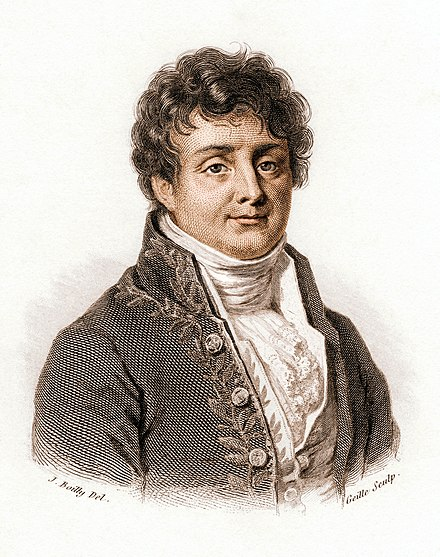
\includegraphics[width=\linewidth]{fourier.jpg}
\end{minipage}

\textbf{\large Notation von Summen und Reihen}
\begin{align*}
	\sum_{n=m}^{N} a_n &= a_m + a_{m+1} + \cdots + a_N, \quad \text{Beispiel:} \;\;\; \sum_{n=1}^{5} n = 1+2+3+4+5 = 15 & \textbf{(Summe)}\\[1ex]
	\sum_{n=m}^{\infty} a_n &= \lim_{N \rightarrow \infty} \sum_{n=m}^{N} a_n = \underbrace{a_m + a_{m+1} + a_{m+2} + \cdots}_{\text{konvergierende unendliche Summe}} , \quad \text{Bsp.:} \;\;\; \sum_{n=0}^{\infty} \left(\frac{1}{2}\right)^n = 1 + \frac{1}{2} + \frac{1}{4} + \cdots = 2 & \textbf{(Reihe)}
\end{align*}

\textbf{\large Reelle Fourierreihe}

Eine periodische Funktion $f: [0; T) \mapsto \mathbb{R}$ mit Periode $T$ lässt sich durch die Reihe
\begin{align*}
	f(t) \;\;=\;\; \underbrace{A_0}_{\text{Gleichwert}} + \sum_{n=1}^\infty \left(A_n \cos\left(2\pi \frac{n}{T} \cdot t\right) + B_n \sin\left(2\pi \frac{n}{T} \cdot t\right)\right) \quad \text{exakt beschreiben}.
\end{align*}
\begin{minipage}[t]{0.49\linewidth}
	\textbf{\large Die komplexen Zahlen $\mathbb{C}$}
	\begin{enumerate}[label={...}]
		\item erweitern die reellen Zahlen ($\mathbb{R} \subset \mathbb{C}$) um eine imaginäre Achse.
		\item können in der \textit{komplexen Zahlenebene} als Vektoren dargestellt werden.
		\item können mithilfe der Eulerschen Formel mit Polarkoordinaten beschrieben werden.
	\end{enumerate}
%	\vspace*{-1ex}
	\begin{center}
		\begin{tikzpicture}[scale=1.7]
			\draw[line width=.5mm, ->] (-1.5,0) -- (1.5, 0) node[right=1ex] {Re};
			
			\draw[line width=1mm] (-1, -0.05) -- ++(0,0.1) node[below left] {$-1$};
			\draw[line width=1mm] (1, -0.05) -- ++(0,0.1) node[below right] {$1$};
			
			\draw[ultra thin, gray] (-1.5,-1.5) grid (1.5,1.5);
			\draw[line width=.5mm, ->] (0,-1.5) -- (0, 1.5) node[above=1ex] {Im};
			
			\draw[line width=1mm] (-0.05, -1) -- ++(0.1, 0) node[below right] {$-i$};
			\draw[line width=1mm] (-0.05, 1) -- ++(0.1, 0) node[above right] {$i$};
			
			\draw[dashed, thick] (0,0) circle (1);
			\draw[ultra thick, ->] (0,0) -- (50:0.95);
			\draw[ultra thick, ->] (1,0) arc (0:40:1);
			\node at (1.1, 0.35) {$\mathbf{x}$};
			
			\node[fill=white, inner sep=1mm, above right=.5ex] at (50:1) {$\mathbf{e^{ix} = \cos x + i \sin x}$};
		\end{tikzpicture}
	\end{center}
\end{minipage}\hfill
\begin{minipage}[t]{0.49\linewidth}
	\textbf{\large Komplexe Zeiger}
	(mit konstanter Frequenz um den Ursprung rotierender Pfeil)
	\begin{enumerate}[label={...}]
		\item können durch eine \textit{Anfangskonfiguration} $C_n \in \mathbb{C}$ und eine \textit{Frequenz} $f_n \in \mathbb{R}$ eindeutig beschrieben werden.
		\item können durch Aufsummieren aneinandergehängt werden $\rightarrow$ Idee der komplexen Fourierreihe.
	\end{enumerate}
	
	\begin{center}
		\begin{tikzpicture}[scale=1.5]
			\draw[line width=.5mm, ->] (-2.5,0) -- (2.5, 0) node[right=1ex] {Re};
			\draw[ultra thin, gray] (-2.5,-1.5) grid (2.5,1.5);
			\draw[line width=.5mm, ->] (0,-1.5) -- (0, 1.5) node[above=1ex] {Im};
			
			\draw[dashed, thick] (0,0) circle (2);
			\draw[ultra thick, ->] (0,0) -- (20:2) node[right] {$C_1$};
			
			\draw[ultra thick, green!50!black, ->] (20:1) arc (20:48:1) node[midway, right] {$x$};
			\draw[ultra thick, green!50!black, ->] (0,0) -- (50:2) node[above right, fill=white] {$C_1 \cdot e^{i x}$};
			
			\draw[ultra thick, red!50!black, ->] (20:.8) arc (20:158:.8) node[fill=white, midway, above, sloped] {nach $t$s...};
			\draw[ultra thick, red!50!black, ->] (0,0) -- (160:2) node[above left, fill=white] {$C_1 \cdot e^{i 2\pi f_1 t}$};
			
			\draw[ultra thick, red!50!black, ->] (160:2) ++(-70:0.2) -- ++(-70:1.8) node[below, fill=white] {$C_1 \cdot e^{i 2\pi f_1 t} + C_2 \cdot e^{i 2\pi f_2 t}$};
			
			\draw[ultra thick, red!50!black, ->] (160:2) ++(-70:2) ++(20:0.2) -- ++(20:1.5);
			\draw[ultra thick, red!50!black, ->] (160:2) ++(-70:2) ++(20:1.7) ++(-10:0.1) -- ++(-10:0.9);
			\draw[ultra thick, red!50!black, ->] (160:2) ++(-70:2) ++(20:1.7) ++(-10:1) ++(-110:0.1) -- ++(-110:0.5) node[below, fill=white] {$\cdots \; + C_n \cdot e^{i 2\pi f_n t}$};
		\end{tikzpicture}
	\end{center}
\end{minipage}
\end{document}
